\documentclass{article} [10pt] % Comment this line out
                                                          % if you need a4paper
                                                          % paper

%\IEEEoverridecommandlockouts                              % This command is only
                                                          % needed if you want to
                                                          % use the \thanks command
%\overrideIEEEmargins
% See the \addtolength command later in the file to balance the column lengths
% on the last page of the document



%=====================PACKAGES======================
% The following packages can be found on http:\\www.ctan.org
%-----------------graphics related---------------------
\usepackage{graphics} % for pdf, bitmapped graphics files
\usepackage{epstopdf}
 \usepackage{epsfig} % for postscript graphics files
\DeclareGraphicsExtensions{.pdf,.eps,.png,.jpg,.mps}
%\usepackage{minibox}
%\usepackage{subfigure}
\usepackage{tikz}
\usetikzlibrary{matrix,chains,positioning,decorations.pathreplacing,arrows}

%\usetikzlibrary{calc,patterns,decorations.pathmorphing,decorations.markings}
%\usepackage{pgfplots}
\setlength{\unitlength}{1cm}
%-------------------layout related-------------------
%\usepackage{cite}
\usepackage{verbatim}
\usepackage{enumerate}
\setlength\parindent{0pt}
\setlength{\parskip}{.25cm}
%-------------------------Math related-------------------------------
%\usepackage{mathptmx} % assumes new font selection scheme installed
\usepackage{times} % assumes new font selection scheme installed
\usepackage{amsmath} % assumes amsmath package installed
\usepackage{amssymb}  % assumes amsmath package installed
\usepackage{empheq}
%\usepackage{algorithm2e}
%\usepackage{algorithm} 
%\usepackage{algpseudocode}
%\usepackage{mathrsfs}
\usepackage{amsthm}
\usepackage{cleveref}
%\newtheoremstyle{definition}
\newtheorem{defi}{Definition}
\newtheorem{asmp}{Assumption}
%-------------------------------------------
%\theoremstyle{plain}
\newtheorem{thm}{Theorem}
\newtheorem{lma}{Lemma}
\DeclareMathOperator{\fl}{fl}
\DeclareMathOperator{\card}{card}
% Comment out the next line to get single spacing
%=====================TITLE======================
\title{Back propagation algoirthm}
\author{Zhe Feng}
\date{\today}


\graphicspath{{Figures/}}

\begin{document}
\noindent
\maketitle
\section{Introduction}
Deep learning is the hottest topic in AI these days. Convolution neural network (CNN) is widely used in image recognition and gained huge success, recurrent neural networks (RNN) used in sequential data prediction and achieved unprecedented performance in automatic speech recognition (ASR) and automatic translation. Behind all these success, is an algorithm that is developed 1960s, independently from researchers in different disciplines, and its name is back propagation.
Back propagation lays in the heart of artificial neural networks, whether it's a simple network with one hidden layer or a complex CNNs, they all use back propagation to calculate the gradient (with different variations). Of course, these days to use complicated neural networks, you don't need to know detail about how back propagation work. However, as a personal interest, I decided to have a proper understanding of how it works and appreciate its beautiful mathematical structure.


\section{Problem Description}	\label{sec:problem_ddescription}
Essentially, given a feature vector $x$ of dimension $n_x$ and a target vector $y$ with dimension $y_{n_y}$ neural network will try to predict and approximate it with $\hat{y}$ which is the output from our neural network. A general neural network can be described by the following equations:

\begin{align}
	&\hat{y}_k := z^L_k \text{ for } k \in \{1, \cdots, n_y\} \label{eq:output} \\
	&z^\ell_k := \sigma^\ell (m^\ell_k) \text{ for } \ell \in \{2, \cdots, L\} \label{eq:layeroutput} \\
	&m^\ell_k := \sum^{n_{\ell-1}}_i w^\ell_{ik}z^{\ell-1}_i \text{ for } k \in \{2, \cdots, n_{\ell}\} \label{eq:netin}\\ 
	&z^1_k := x_k \text{ for } k \in \{1, \cdots, n_x\} \label{eq:input}
\end{align}
where
\begin{enumerate}
	\item $z^\ell \in \mathbb{R}^{n_\ell}$ is the net output of the $\ell^{th}$ layer (so the $L$ is the output layer of the net.
	\item $m^\ell \in \mathbb{R}^{n_\ell}$ is the net input of the $\ell^{th}$ layer.
	\item $w^\ell := [w^\ell_{11}, w^\ell_{12}, \cdots,w^\ell_{n_{\ell-1}1}, \cdots,w^\ell_{n_{\ell-1}n_\ell}]^\top \in \mathbb{R}^{n_{\ell-1}n_\ell}$ is the weight parameters at layer $\ell$, where $w^\ell_{ij}$ is the weight at layer $\ell$ connect node $i$ at layer $\ell-1$ to node $j$ in layer $\ell$. Note that we don't have $w^1$ since the 1st layer is the input layer.
	\item $W^\ell := \begin{bmatrix}
				w_{11}^\ell &w_{12}^\ell &\cdots &w_{1n_{\ell-1}}^\ell\\
				w^\ell_{21} &\ddots \\
				\vdots,\\
				w^\ell_{n_{\ell}1} &&&w^\ell_{n_{\ell}n_{\ell-1}}
				\end{bmatrix} \in \mathbb{R}^{n_\ell \times n_{\ell-1}}$ is the weight matrix at layer $\ell$, this is for the convenience of notation later.
	\item $\sigma^\ell(x)$ is the activation function at the $\ell^{th}$ layer (in most cases are sigmoid function, hence the symbol $\sigma$).
\end{enumerate}

The 4 equation description is very simple and elegant: equation \eqref{eq:output} essentially just say the last layer's output $z^L$ is our target estimation $\hat{y}$ and equation \eqref{eq:input} state that the first layer's output $z^1$ is the input feature variable $x$. With the start and the end defined, equation \eqref{eq:netin} and \eqref{eq:layeroutput} are recursive definition of the layers. This is illustrated in the following example plot:

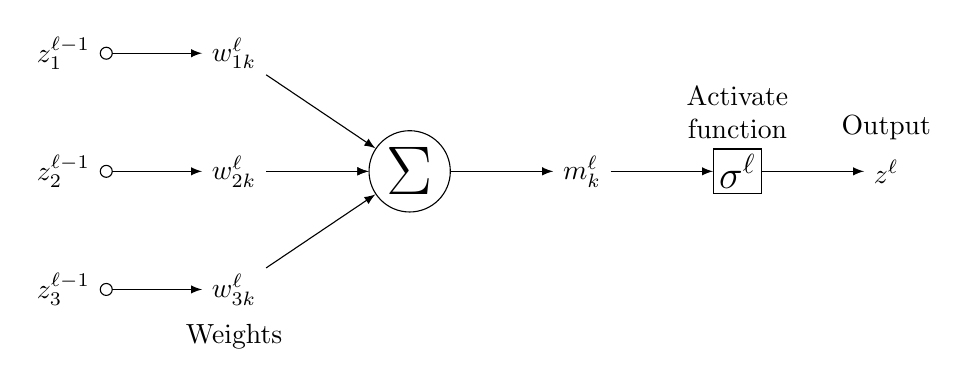
\begin{tikzpicture}[
	init/.style={
	  draw,
	  circle,
	  inner sep=2pt,
	  font=\Huge,
	  join = by -latex
	},
	squa/.style={
	  draw,
	  inner sep=2pt,
	  font=\Large,
	  join = by -latex
	},
	start chain=2,node distance=13mm
]

% z_1
\begin{scope}[start chain=1]
\node[on chain=1] at (0,1.5cm) 
  (z1) {$z^{\ell-1}_1$};
\node[on chain=1,join=by o-latex] 
  (w1) {$w^\ell_{1k}$};
\end{scope}

% z_2
\begin{scope}
\node[on chain=2] 
  (z2) {$z^{\ell-1}_2$};
\node[on chain=2,join=by o-latex] 
 (w2) {$w^\ell_{2k}$};
\end{scope}

% z_3
\begin{scope}[start chain=3]
\node[on chain=3] at (0,-1.5cm) 
  (z3) {$z^{\ell-1}_3$};
\node[on chain=3,label=below:Weights,join=by o-latex] 
  (w3) {$w^\ell_{3k}$};
\end{scope}


% input bracket
%\draw[decorate,decoration={brace,mirror}] (z1.north west) -- node[left=10pt] {Previous layer outputs} (z3.south west);

\begin{scope}
\node[on chain=2,init] (sigma)
  {$\displaystyle\Sigma$};
  
\node[on chain=2,join=by -latex]  (m)
  {$m^\ell_k$};
  
\node[on chain=2,squa,label=above:{\parbox{2cm}{\centering Activate \\ function}}]   
  {$\sigma^\ell$};
\end{scope}

%\node[label=above:\parbox{2cm}{\centering Bias \\ $b$}] at (sigma|-w1) (b) {};

\draw[-latex] (w1) -- (sigma);
\draw[-latex] (w2) -- (sigma);
\draw[-latex] (w3) -- (sigma);
%\draw[o-latex] (b) -- (sigma);

\node[on chain=2,label=above:Output,join=by -latex] 
  {$z^{\ell}$};


\end{tikzpicture}




Note that the ultimate goal is to tune the weights and make sure that the error is minimised. So our cost function would be:
\begin{align*}
	\text{min}_w &Q(y; w) := \frac{1}{N} \sum_i^N \frac{1}{2}\| \hat{y}^{(i)} - y^{(i)} \|^2 \\
	&\text{s.t. \cref{eq:output,eq:input,eq:netin,eq:layeroutput}} \\
	\text{where } &w := \{w^2 \cdots w^L\}
\end{align*}

\section{Back propagation algorithm}
In general, for most optimisation algoirthm, the bottomline comes to find a stationary point where the derivative is zero, that is:
\begin{align}
	w^* \text{ such that }\nabla_wQ = 0
\end{align}
And that is what makes optimisation of neural network hard: neural networks' definition function is a recursive definition and finding gradient of it is very challenging. Back propagation essentially leverage chain rule in calculus to recursively propagate the error gradient backwards from the last output layer to the first input layer.

\subsection{Output layer delta}
Consider the weights $W^L$ in the output layer, the partial derivative to those weights are:
\begin{align} \label{eq:output_delta}
\boxed{
	\frac{\partial Q}{\partial w^L_{ij}} = \frac{\partial Q}{\partial z^L_{j}}
							\frac{\partial z^L_{j}}{\partial m^L_{j}}
							\frac{\partial m^L_{j}}{\partial w^L_{ij}}
}
\end{align}
This is done by using chain rule, and we know that $w^L_{ij}$ will only contribute to the $j^{th}$ output $y_j=z^L_j$
.

\subsubsection{Find the term   $\frac{\partial z^L_{j}}{\partial m^L_{j}}$}
Now for $\frac{\partial z^L_{j}}{\partial m^L_{j}}$, we can see:
\begin{align} \label{eq:dzdm_sigmoid_derivative}
\boxed{
	\frac{\partial z^L_{j}}{\partial m^L_{j}} = \frac{\partial}{\partial m^L_{j}}\sigma^L(m^L_{j}) = {\sigma^L}^\prime(m^L_{j})
}
\end{align}
where
\begin{align}
	{\sigma^L}^\prime(m^L_{j}) := \frac{d}{dm^L_{j}}\sigma^L(m^L_{j})
\end{align}
One special case, is when the activation function is the logistic sigmoid function:
\begin{align}
	&\sigma^L(m) := \frac{1}{1+e^{-m}} \\
	\therefore \ &{\sigma^L}^\prime(m) = \sigma^L(m)(1-\sigma^L(m))
\end{align}
detailed derivation can be done easily using chain rule.

\subsubsection{Find the term $\frac{\partial m^L_{j}}{\partial w^L_{ij}}$}
Recall the definition of $m^L$, \eqref{eq:netin}, then the next term is easy:
\begin{align}\label{eq:dmdw_z}
\boxed{
	\frac{\partial m^L_{j}}{\partial w^L_{ij}} = z^{L-1}_i
}
\end{align}
or in a more general form:
\begin{align}\label{eq:dmdw_z}
	\frac{\partial m^\ell_{j}}{\partial w^\ell_{ij}} = z^{\ell-1}_i
\end{align}

Put things together and substitute \eqref{eq:dzdm_sigmoid_derivative}  and \eqref{eq:dmdw_z} back to \eqref{eq:output_delta}, we have
\begin{align}
	\frac{\partial Q}{\partial w^L_{ij}} = \frac{\partial Q}{\partial z^L_{j}}
							{\sigma^L}^\prime(m^L_{j}) 
							z^{L-1}_i
\end{align}
wich in a more compact vector form, we can write it as 
\begin{align}
	\nabla_{w^L} Q = (\nabla_{z^L}Q \odot {\sigma^L}^\prime(m^L)) \otimes z^{L-1}
\end{align}
where
\begin{align}
	\nabla_{w^L} Q = \begin{bmatrix}
		\frac{\partial Q}{\partial w^L_{11}} \\
		\frac{\partial Q}{\partial w^L_{12}} \\
		\vdots\\
		\frac{\partial Q}{\partial w^L_{n_{\ell-1}n_\ell}}
	\end{bmatrix}
\end{align}

For implementation and notation convenience, we can also re-write the above equation as
\begin{align} \label{eq:delta_w_out}
\boxed{
	\Delta W^L = z^{L-1}(\nabla_{z^L}Q \odot {\sigma^L}^\prime(m^L))^\top
}
\end{align}
where
\begin{align}
	\Delta W^L &= \begin{bmatrix}z^{L-1}_1\\ z^{L-1}_2\\ \vdots \\z^{L-1}_{n_{L-1}}\end{bmatrix}
	\begin{bmatrix}   \frac{\partial Q}{\partial z^L_{1}}{\sigma^L}^\prime(m^L_{1}),
	\frac{\partial Q}{\partial z^L_{2}}{\sigma^L}^\prime(m^L_{2}), \cdots
	\frac{\partial Q}{\partial z^L_{n_L}}{\sigma^L}^\prime(m^L_{n_L})
	\end{bmatrix}\\
	 &= \begin{bmatrix}
				\frac{\partial Q}{\partial w^L_{11}} &\frac{\partial Q}{\partial w^L_{12}} &\cdots \\
				\frac{\partial Q}{\partial w^L_{21}} &\ddots \\
				\vdots,\\
				\end{bmatrix} \in \mathbb{R}^{n_{\ell-1}\times n_\ell}
\end{align}
which can then be easily plug in to the update equation \boxed{W^L -=\eta\Delta W^L} and $\eta$ is the learning rate.


\subsubsection{$\delta$ notation}
To make sense of the backpropagation, we use $\delta$ notation to denote the error delta for a particular node. Define:
\begin{align}
	\delta^L := \nabla_{z^L}Q \odot {\sigma^L}^\prime(m^L)
\end{align}
where
\begin{align}
	\delta^L = \begin{bmatrix} \delta^L_1\\ \vdots\\ \delta^L_{n_L}\end{bmatrix} \\ 
	\text{and } 
	\delta^L_j =\frac{\partial Q}{\partial z^L_{j}}{\sigma^L}^\prime(m^L_{j}) \label{eq:node_delta_output}
\end{align}
or more generally:
\begin{align}
	\delta^\ell_j := \frac{\partial Q}{\partial z^\ell_j}\frac{\partial z^\ell_j}{\partial m_j}
\end{align}
Then equation \eqref{eq:delta_w_out} can be rewritten as:
\begin{align}
	\Delta W^L = (z^{L-1}){\delta^L}^\top
\end{align}

\subsection{Hidden layers deltas}
Now for hiddenlayers, similar principle applies:
\begin{align} \label{eq:hidden_delta}
\boxed{
	\frac{\partial Q}{\partial w^\ell_{ij}} = \sum_k^{n_{\ell+1}}\frac{\partial Q}{\partial z^{\ell+1}_{k}}
							\frac{\partial z^{\ell+1}_{k}}{\partial m^{\ell+1}_{k}}
							\frac{\partial m^{\ell+1}_{k}}{\partial z^\ell_j}
							\frac{\partial z^\ell_j}{\partial m^\ell_{j}}
							\frac{\partial m^\ell_{j}}{\partial w^\ell_{ij}}
\text{ for } \ell \in \{2, \cdots, L-1\}
}
\end{align}
This holds because it follows the chain rule for partial differentiation in the following form:
\begin{align*}
	\frac{\partial f(g_1(x), g_2(x), \cdots g_n(x))}{\partial x} = \sum_i^n \frac{\partial f}{\partial g_i}\frac{d g_i(x)}{dx}
\end{align*}
The key difference here is for hidden layers, the partial derivative of weight $w^\ell_{ij}$ will affect all the nodes in $\ell+1$ layer (unlike in output layer $L$, where $w^L_{ij}$ will only affect $j^{th}$ node, which is $z^L_j$), hence the sum over all the partial derivatives of $\ell+1$ layer nodes: $\frac{\partial Q}{\partial w^\ell_{ij}} = \sum_k^{n_{\ell+1}}\frac{\partial Q}{\partial z^{\ell+1}_{k}}\frac{\partial z^{\ell+1}_{k}}{\partial w^\ell_{ij}}$.


\subsubsection{Recursively define $\delta^\ell$ through back propagation}
It is easy to see that:
\begin{align}
\frac{\partial Q}{\partial z^{\ell+1}_{k}}\frac{\partial z^{\ell+1}_{k}}{\partial m^{\ell+1}_{k}} = \frac{\partial Q}{\partial z^{\ell+1}_{k}}{\sigma^{\ell+1}}^\prime(m^{\ell+1}_{k}) = \delta^{\ell+1}_k
\end{align}
and when $\ell=L-1$, from equation \eqref{eq:node_delta_output} we have $\delta^L_j$. It is also easy to see that:
\begin{align}
	\frac{\partial m^{\ell+1}_{k}}{\partial z^\ell_j} = w^{\ell+1}_{jk}
\end{align}
from the definition in equation \eqref{eq:netin}. Through similar logic in deducing output layer delta, with equations \eqref{eq:dzdm_sigmoid_derivative}  and \eqref{eq:dmdw_z}, we can write equation \eqref{eq:hidden_delta} as:
\begin{align}
	\frac{\partial Q}{\partial w^\ell_{ij}} = \sum_k^{n_{\ell+1}}\delta^{\ell+1}_kw^{\ell+1}_{jk}
							{\sigma^{\ell}}^\prime(m^{\ell}_j)z^{\ell-1}_i
\text{ for } \ell \in \{2, \cdots, L-1\}
\end{align}
since we can also write the above as:
\begin{align}
	\frac{\partial Q}{\partial w^\ell_{ij}} =  \frac{\partial Q}{\partial z^\ell_j}\frac{\partial z^\ell_j}{\partial m^\ell_j}\frac{\partial m^\ell_j}{\partial w^\ell_{ij}}
\text{ for } \ell \in \{2, \cdots, L-1\}
\end{align}
and we can see $\frac{\partial m^\ell_j}{\partial w^\ell_{ij}}=z^{\ell-1}_i$:
\begin{align}
\boxed{
	\delta^\ell_j :=  \frac{\partial Q}{\partial z^\ell_j}\frac{\partial z^\ell_j}{\partial m^\ell_j} = \sum_k^{n_{\ell+1}}\delta^{\ell+1}_kw^{\ell+1}_{jk}{\sigma^{\ell}}^\prime(m^{\ell}_j)
} \\
\boxed{
	\therefore \text{in vector form }  \delta^\ell := W^{\ell+1}{\delta^{\ell+1}} \odot {\sigma^{\ell}}^\prime(m^{\ell})
}
\end{align}
Note that when $\ell=L-1$, the $\delta^{\ell+1}=\delta^L$ which is the output layer nodes' deltas defiend in equation \eqref{eq:node_delta_output}.

So now for hidden layer, we can have the same form of definition as for output layer:
\begin{align} \label{eq:delta_w_hidden}
\boxed{
	\Delta W^\ell = z^{\ell-1}{\delta^{\ell}}^\top
}
\end{align}
\newpage
\subsection{The back propagation algorithm}
Now we have all the ingradient to summarise our back propagation algorithm:
\begin{enumerate}
	\item run feedforward through the neuralnet work, calculate all $m^\ell$, $z^\ell$ and consequently $\hat{y}$.
	\item back propagate the error, calculate $\Delta W^\ell$ for all $\ell \in \{2, \cdots, L\}$.
	\item update all $W^\ell$ with 
	\begin{align}
		\boxed{W^\ell = W^\ell - \eta\Delta W^\ell \text{ for } \ell \in \{2, \cdots, L\}}
	\end{align}
	where 
%	\begin{subequations}
	\begin{empheq}[box=\fbox]{align}
		\Delta W^\ell &= z^{\ell-1}{\delta^{\ell}}^\top  \\
		\delta^\ell &= W^{\ell+1}{\delta^{\ell+1}} \odot {\sigma^{\ell}}^\prime(m^{\ell}) \text{ for } \ell \in \{2,\cdots, L-1\}\\
		\delta^L &= \nabla_{z^L}Q \odot {\sigma^L}^\prime(m^L)
	\end{empheq}
%	\end{subequations}
	\item Repeat till converge ($\nabla_wQ \leq \epsilon$).
\end{enumerate}
Note that we still haven't discussed bias at each layer $b^\ell$ yet. It is actually very simple, it can be shown that 
\begin{align}
	\boxed{\Delta b^\ell = \delta^\ell \text{ for } \ell \in \{2, \cdots, L\}}
\end{align}
therefore bias $b^\ell$ can be updated by 
\begin{align}
	\boxed{b^\ell = b^\ell - \eta\Delta b^\ell \text{ for } \ell \in \{2, \cdots, L\}}
\end{align}
\end{document}
%%%%%%%%%%%%%%%%%%%%%%%%%%%%%%

































